%!TEX program = xelatex
\documentclass{beamer}

\usepackage[english]{babel}

\usepackage{graphicx,hyperref,url, materialbeamer}
\usepackage{braket}
%\usepackage{euler}
\usepackage{listings}
\usepackage{mathrsfs}


\graphicspath{ {./figs/} }
\setbeamercovered{transparent}
\lstdefinestyle{customsql}{
  belowcaptionskip=1\baselineskip,
  breaklines=true,
  xleftmargin=\parindent,
  language=SQL,
  showstringspaces=false,
  basicstyle=\footnotesize\ttfamily,
  keywordstyle=\bfseries\color{green!40!black},
  commentstyle=\itshape\color{purple!40!black},
  identifierstyle=\color{blue},
  stringstyle=\color{orange},
}
\lstset{escapechar=@,style=customsql}



\usefonttheme{professionalfonts} % using non standard fonts for beamer
%\usefonttheme{serif}

% The title of the presentation:
%  - first a short version which is visible at the bottom of each slide;
%  - second the full title shown on the title slide;
\title[Study of the subcommittee on Patents, Trademarks, and Copyrights]{}

% Optional: a subtitle to be displayed on the title slide
\subtitle[Study of the subcommittee on Patents, Trademarks, and Copyrights]{
Study of the subcommittee on Patents, Trademarks, and Copyrights}

% The author(s) of the presentation:
%  - again first a short version to be displayed at the bottom;
%  - next the full list of authors, which may include contact information;
\author[G. Legnaro]{
G. Legnaro} 
  
%\titlegraphic{\includegraphics[width=\textwidth]{atac-logo}}

% The institute:
%  - to start the name of the university as displayed on the top of each slide
%    this can be adjusted such that you can also create a Dutch version
%  - next the institute information as displayed on the title slide
\institute[Sapienza Università di Roma]{
Intellectual Property Competition and Data Protection Law\\
  Master Degree in Data Science \\
  Sapienza Università di Roma}

% Add a date and possibly the name of the event to the slides
%  - again first a short version to be shown at the bottom of each slide
%  - second the full date and event name for the title slide
\date[\today]{
 \today}




\providecommand{\di}{\mathop{}\!\mathrm{d}}
\providecommand*{\der}[3][]{\frac{d\if?#1?\else^{#1}\fi#2}{d #3\if?#1?\else^{#1}\fi}} 
 \providecommand*{\pder}[3][]{% 
    \frac{\partial\if?#1?\else^{#1}\fi#2}{\partial #3\if?#1?\else^{#1}\fi}% 
  }
\begin{document}

\begin{frame}
  \titlepage
\end{frame}

\begin{frame}
  \frametitle{Table of Contents}


  \tableofcontents
\end{frame}

%!TEX root = presentazioneNBD.tex

\setlength{\parskip}{\baselineskip} 
\section{Definitions and literature}
\begin{frame}[t]
\frametitle{Definitions and literature}
\begin{block}{What is going to be explained?}
	\begin{itemize}
		\item Thesis
		\item Single Commodity Flow Problems
		\item Multicommodity Flow Problems
		\item Prior work on max-flows and min-cuts for multicommodity flow problems
		\item Max-flow min-cut results
		\item Applications to Approximation Algorithms
		\item Subsequent Work
	 \end{itemize} 
\end{block}
\end{frame}

\begin{frame}
%\subsection{Thesis}
\frametitle{Thesis}
Relationship between maximum flow and minimum cut in multicommodity flow problem

Previous Literature:\\
Ford and Fulkerson [1956]
max-flow and min-cut always equal in 1-commodity flow problems
\end{frame}


\begin{frame}
%\subsection{Single Commodity Flow Problems}
\frametitle{Single Commodity Flow Problems}
1-commodity flow problems
\begin{itemize}
	\item $n$ nodes $V$
	\item $m$ edges $E$
	\item non negative capacity $C(e)$ for each $e \in E$. 
	% Maximum amount of flow that can pass through the edge (if not specified, we assume that the edges are undirected)
	\item nodes designation: 
	\begin{itemize}
		\item \textit{source} $s$
		\item \textit{sink} $t$
	\end{itemize}
\end{itemize}
\end{frame}


\begin{frame}
\frametitle{Single Commodity Flow Problems}
\textit{Objective:}\\
to route as much flow as possible from the source to the sink without violating the capacity of any edge.

\textit{max-flow:}\\
maximum amount of flow that can be routed.

\textit{min-cut:}\\
minimum amount of capacity that needs to be removed from the network in order to disconnect the source from the sink. Formally:
$$\min_{ \{ U \subset V | s \in U, t \in \bar{U} \} } \sum_{e \in \langle U, \bar{U} \rangle } C(e)$$
%U is any subset of V that contains the source but not the sink
%$\bar{U} = V - U$ the set of nodes not in U
%$\langle U, \bar{U} \rangle$  set of edges that link a node in U to a node in $\bar{U}$ 
\end{frame}

\begin{frame}
\frametitle{Single Commodity Flow Problems}
\textit{cut of the network:}\\
set of edges from any set $U$ to $\bar{U}$ since the removal of those edges separates $U$ from the rest of the network.

\textit{min-cut 1-commodity flow problem is always an upper bound on the max-flow. Why?}\\
For any $U \subseteq V$ that contains the source but not the sink, all flow from $s$ to $t$ must be routed through edges in  $\langle U, \bar{U} \rangle $. Hence, the total flow is limited by the capacity in the min-cut.
\end{frame}


\begin{frame}[c]
\frametitle{Single Commodity Flow Problems}
	\begin{figure}
		\centering
		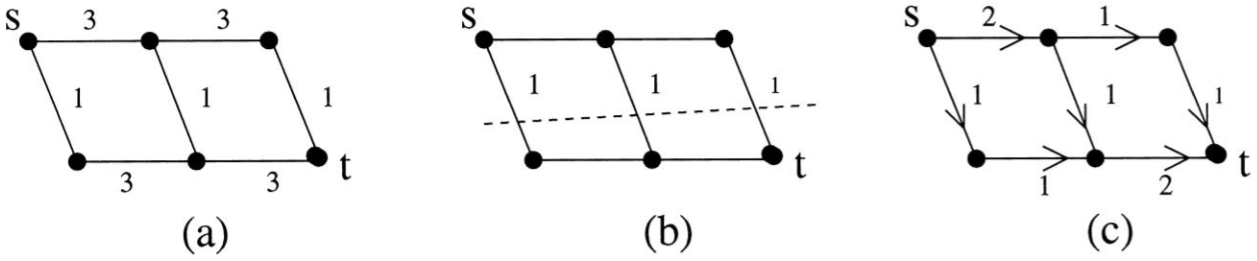
\includegraphics[width=\textwidth]{figs/1-commodity_flow_problem.png}
		\caption{Solution to a 1-commodity flow problem}
		\end{figure}
\end{frame}


\begin{frame}
%\subsection{Multicommodity Flow Problems}
\frametitle{Multicommodity Flow Problems}
\begin{center}
\textit {k $ \ge 1$}\\
\end{center}

$k$ number of commodities, each with source $s_i$, sink $t_i$ and demand $D_i$

\textit{Objective:}\\
simultaneously route $D_i$ units of commodity $i$ from $s_i$ to $t_i$ for each $i$ so that the total amount of all commodities passing through any edge is no greater than its capacity.
%undirected edges the sum of the flow in both directions cannot exceed the capacity of the edge.
%useful to maximize the amount of flow that can be routed for each commodity.
\end{frame}


\begin{frame}
\frametitle{Multicommodity Flow Problems}
\textit{concurrent max-flow:}\\
maximize a common fraction $f$ of each commodity that is routed. In other words the maximum value of $f$ such that $fD_i$ units of commodity $i$ can be simultaneously routed for each $i$ without violating any capacity constraints.

\textit{fairness property:}\\
ensures that proportionally more of one commodity will not be routed at the expense of another.

\textit{min-cut (a.k.a sparset cut $\mathscr{S}$):}\\
the minimum over all cuts of the ratio of the capacity of the cut to the demand of the cut.
\end{frame}

\begin{frame}
\frametitle{Multicommodity Flow Problems}
$$ \mathscr{S} = \underset{U \subseteq V }{min} \frac{C(U,\bar{U})}{D(U,\bar{U})}, $$
where 
$$ C(U,\bar{U}) = \sum_{e \in \langle U, \bar{U} \rangle} C(e) $$
is the sum of capacities of the edges linking $U$ to $\bar{U}$ and 
$$ D(U,\bar{U}) = \sum_{ \{ i | s_i \in U \land t_i \in \bar{U}\quad or \quad t_i \in U \land s_i \in \bar{U} \} } D_i $$
is the sum of the demands whose source and sink are on opposite sides of the cut that separates $U$ from $\bar{U}$
\end{frame}

\begin{frame}[c]
\frametitle{Multicommodity Flow Problems}
	\begin{figure}
		\centering
		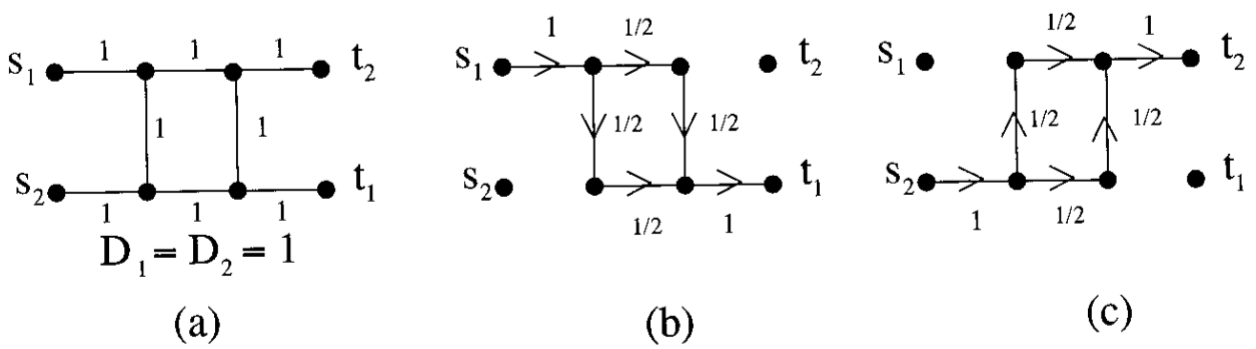
\includegraphics[width=\textwidth]{figs/2-commodity_flow_problem.png}
		\caption{Solution to a 2-commodity flow problem}
	\end{figure}
\end{frame}


\begin{frame}
\frametitle{Multicommodity Flow Problems}
Check that the \textit{max-flow} is always upper bounded by the \textit{min-cut} for any multicommodity flow problem. Let $i_1,i_2,i_3,\dots,i_r$ denote the commodities  whose source and sink are separated by some cut $\langle U, \bar{U} \rangle$
$$	\sum_{j=1}^{r} fD_{i_{j}} \le C(U, \bar{U})	$$
Since
$$	\sum_{j=1}^{r} D_{i_{j}} = D(U, \bar{U})	$$
this means that
$$	f \le \frac{C(U, \bar{U})}{D(U, \bar{U})}	$$
%the max flow is upper bounded by the min-cut
\end{frame}


\begin{frame}
%\subsection{Prior work on max-flows and min-cuts for multicommodity flow problems}
\frametitle{Prior work on max-flows and min-cuts for multicommodity flow problems}
Schrijver [1990]\\
If the graph formed by the set of demands does not contain either three disjoint edges or a triangle and a disjoint edge\\
\quad ---> \quad \textit{max-flow and min-cut are equal}

Example: when there is a commodity for every pair of nodes and all demands are equal, the max-flow and min-cut are equal provided that the dual of the flow problem satisfies a certain cut condition.

\textit{general networks}\\  
The max-flow is within a factor of $k$ of the min-cut since each commodity can be optimized separately using 1/k of the capacity of each edge.
\end{frame}

\begin{frame}
\frametitle{Prior work on max-flows and min-cuts for multicommodity flow problems}
	\begin{figure}
 		\centering
    		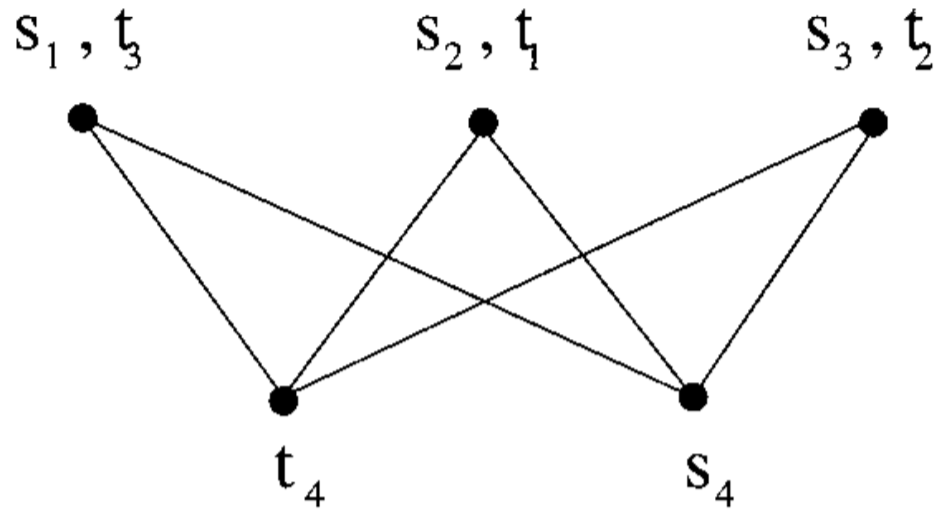
\includegraphics[width=0.5\textwidth]{figs/3-Okamura_Seymour.png}
		\caption{Okamura-Seymour [1981] with max-flow=3/4 and min-cut=1}
	\end{figure}
\end{frame}


\begin{frame}
%\subsection{Max-flow min-cut results}
\frametitle{Max-flow min-cut results}
	 \textit{UMFP (Uniform Multicommodity Flow Problem)}\\
	 In this kind of flow problem there is a commodity for every pair of nodes and the demand for every commodity is the same. WLOG the demand for every commodity is set to one.
	 %Without Loss Of Generality
\end{frame}

\begin{frame}
\frametitle{Max-flow min-cut results}
\begin{block}{What is going to be proved?}
	\begin{itemize}
		\item An approximate max-flow min-cut theorem for uniform multicommodity flow problems. 
		The max flow is within a $\Theta (\texttt{log} n)$-factor of the min-cut. 
		\item The previous bound is tight in the sense that there exist uniform flow problems for which the max-flow is precisely a factor of $\Theta(\texttt{log}n)$ smaller than the min-cut for any $n$.
		% Also we show that this bound is tight in the sense that there exist uniform flow problems for which the max-flow is precisely a factor of $\Theta(\texttt{log}n)$ smaller than the min-cut for any $n$.
	 \end{itemize} 
\end{block}
\end{frame}


\begin{frame}
\frametitle{Max-flow min-cut results}
What is $\Theta$?\\
For a given function $g(n)$, we denote by $\Theta (g(n))$ the set of functions
\begin{equation*}	
	\begin{split}
		\Theta(g(n)) = \{ f(n) : & \text{ $\exists \quad c_1, c_2 > 0$ and $n_0$ such that} \\
						 & 0 \le c_1 g(n) \le f(n) \le c_2 g(n) \quad \forall n \ge n_0 \}
	\end {split}
\end{equation*}
\end{frame}

\begin{frame}
\frametitle{Max-flow min-cut results}
	\begin{figure}
 		\centering
    		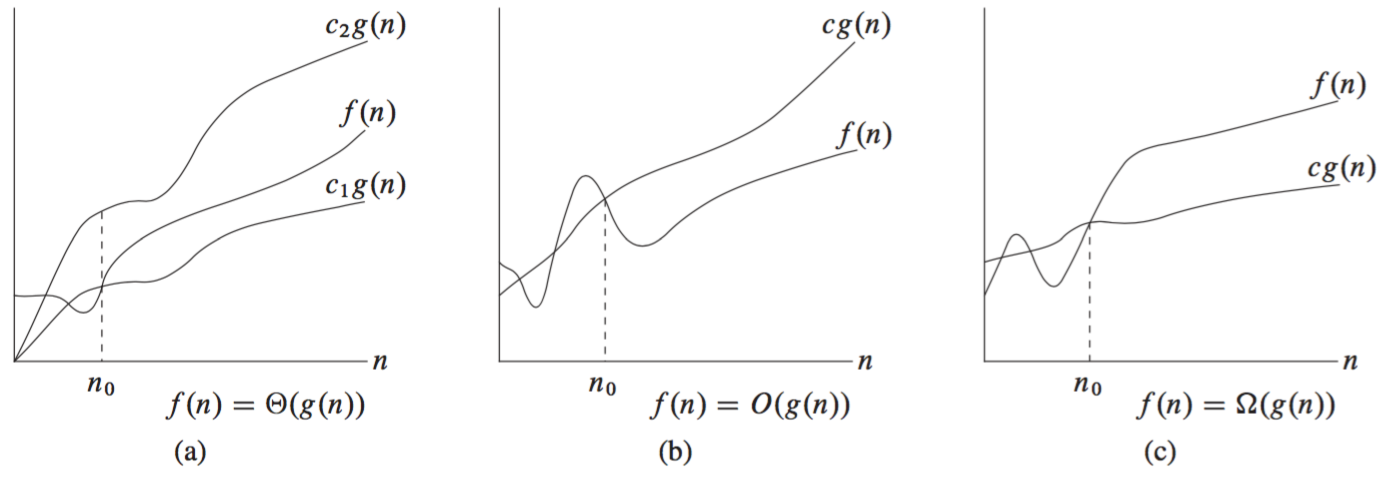
\includegraphics[width=\textwidth]{figs/4-Asymptotic_notation.png}
		\caption{Graphic examples of the $\Theta$, $O$, and $\Omega$  notations. (a) $\Theta$-notation bounds a function to within constant factors. (b) $O$-notation gives an upper bound for a function to within a constant factor. (c) $\Omega$-notation gives a lower bound for a function to within a constant factor.}
%Graphic examples of the $\Theta$, $O$, and $\Omega$  notations. In each part, the value of $n_0$ shown is the minimum possible value; any greater value would also work. (a) $\Theta$-notation bounds a function to within constant factors. We write $f(n) = \Theta (g(n))$ if there exist positive constants $n_0$, $c_1$, and $c_2$ such that at and to the right of $n_0$, the value of $f(n)$ always lies between $c_1 g(n)$ and $c_2 g(n)$ inclusive. (b) $O$-notation gives an upper bound for a function to within a constant factor. We write $f(n) = O(g(n))$ if there are positive constants $n_0$ and $c$ such that at and to the right of $n_0$, the value of $f(n)$ always lies on or below $cg(n)$. (c) $\Omega$-notation gives a lower bound for a function to within a constant factor. We write $f(n) = \Omega (g(n))$ if there are positive constants $n_0$ and $c$ such that at and to the right of $n_0$, the value of $f(n)$ always lies on or above $cg(n)$.
	\end{figure}
\end{frame}



\begin{frame}
%\subsection{Applications to Approximation Algorithms}
\frametitle{Applications to Approximation Algorithms}
In a UMFP we have:\\
\textit{Demand} across a cut $\langle U, \bar{U} \rangle$ 
%is the product of the number of nodes in $U$ and the number of nodes in $\bar{U}$
$$D(U,\bar{U}) = |U||\bar{U}|$$
\textit{Min-cut} of uniform flow problem is
$$ \mathscr{S} = \underset{U \subseteq V}{min} \frac{C(U,\bar{U})}{ |U||\bar{U}|}$$
where $C(U,\bar{U}) = \sum_{e \in \langle U, \bar{U} \rangle } C(e)$.\\
In the case when all capacities are 1, the min-cut is simply
$$ \mathscr{S} = \underset{U \subseteq V}{min} \frac{| \langle U,\bar{U}\rangle |}{ |U||\bar{U}|}$$
\end{frame}

\begin{frame}
\frametitle{Applications to Approximation Algorithms}
\textit{min-cut} is a good measure of the number of edges that need to be removed in order to partition the underlying network into pieces of various sizes.

\textit{Consequence:} able to use our algorithm for finding an approximate min-cut to design the first nontrivial polynomial-time approximation algorithms for several important NP-hard graph partitioning problems.
\end{frame}


\begin{frame}
%\subsection{Subsequent Work}
\frametitle{Subsequent Work}
More literature and results of this paper was published at the first time in an extended abstract of Leighton and Rao [1988].\\

Subsequent work:
\begin{itemize}
	\item Klein et al. [1995] the max-flow is always within an $O(\texttt{log} C \texttt{log} D)$ factor of the min-cut for undirected multicommodity flow problems.
	\item Tragoudas [1990], Plotkin and Tardos [1993] and Garg et al. [1996] have improved the previous bound to $O(\texttt{log}^2 k)$
	\item Linial  et al. [1995] and Aumann and Rabani [1998] established an existentially tight gap of $\Theta(\texttt{log} k)$ with the use of Bourgain's technique with embed spaces on graphs into geometric spaces.
\end{itemize}
\end{frame}	

\begin{frame}
\frametitle{Subsequent Work}
\begin{itemize}	
	\item Garg  et al. [1996] established an $O(\texttt{log} k)$  max-flow min-cut theorem for arbitrary (undirected) multicommodity flow problems where the sum of the flows is maximized. 
	\item Klein et al. [1993] discovered a $\Theta(1)$ max-flow min-cut theorem for uniform multicommodity flow problems in undirected planar graphs and graphs with small excluded minors.
	\item Klein et al. [1997] and Even et al. [1998] $O(\texttt{log}^3 k)$ max-flow min-cut theorem for multicommodity flow problems in directed networks for which the demand from any node u to any node v is equal to the demand from v to u. 
\end{itemize}
\end{frame}





%!TEX root = DPLAW.tex

\setlength{\parskip}{\baselineskip} 
\section{Historical Survey}
\begin{frame}[t]
\frametitle{Early History (Before 1624)}

Oldest example: $14^{th}$ century. Probably the first “patent law”, was enacted in 1474 by the Republic of Venice.

In the $16^{th}$ century, patents were widely used by \textit{German} princes, some of whom had a well-reasoned policy of \textit{granting privileges} on the basis of a careful consideration of the utility and novelty of the inventions and, also, of the burden which would be imposed on the country by \textit{excluding} others from the use of these inventions and by enabling the patentees to \textit{charge higher prices}.

\end{frame}

\begin{frame}
\frametitle{Early History (Before 1624)}
Exclusive privileges were on:
\begin{itemize}
	\item new inventions
	\item skilled crafts imported from abroad
\end{itemize}

Canton Bern in Switzerland granted in 1577 to inventor Zobell a \textit{permanent exclusive privilege}
\end{frame}

\begin{frame}
\frametitle{Early History (Before 1624)}
In France, the persecution of innovators by guilds of craftsmen continued far into the
18th century. 

In 1726, the weavers' guild threatened design printers with severe punishment, including death.

Royal patent privileges were sometimes conferred, not to grant exclusive rights, but to grant permission to do what was prohibited under existing rules.
\end{frame}

\begin{frame}
\frametitle{The Spread of the patent system (1624-1850)}
The Statute of Monopolies is the basis of the present British patent law, and became the model for the laws elsewhere.
\begin{itemize}
	\item 1691 South Carolina - first \textit{general} patent law
	\item 1762 France - edict of King Louis XV did little more than prohibit permanent privileges and provide for inventors’ patents limited to 15 years
    \item 1791 Constitutional Assembly passed a comprehensive patent law, in which the inventor's right in his creation was declared a \textit{property right} based on the \textit{rights of man}
\end{itemize}
\end{frame}

\begin{frame}
\frametitle{The Spread of the patent system (1624-1850)}
\begin{itemize}
	\item 1787 United States of America - Constitution had given Congress the power \textit{to promote the Progress of Science and useful Arts, by securing for limited Times to Authors and Inventors the exclusive Right to their respective Writings and Discoveries}
	\item 1794 Austria (Hofdekret) - announced the establishment of a patent system
\end{itemize}
\end{frame}

\begin{frame}
\frametitle{The rise of an antipatent movement (1850- 1873)}
\begin{itemize}
	\item 1863 Germany - condemned \textit{patents of invention as injurious to common welfare}
	\item 1849, 1851, 1854, and twice in 1863 Switzerland - \textit{economists of greatest competence} had declared the principle of patent protection to be \textit{pernicious and indefensible}
\end{itemize}
\end{frame}

\begin{frame}
\frametitle{The victory of the patent advocates (1873-1910)}
Thanks to the bad crisis, public opinion had turned away from \textit{the pernicious theory of free competition and free trade}
\begin{itemize}
	\item 1874 Britain - drastic reform bill had passed the House of Lords withdrew in the House of Commons
	\item 1877 Germany - uniform patent law for the entire Reich
    \item 1872 Japan - had adopted her first patent law, only to abolish it again in 1873, enacted another law in 1885
\end{itemize}
\end{frame}



%!TEX root = DPLAW.tex

\setlength{\parskip}{\baselineskip} 
\section{Institutional Facts and Problems}
\begin{frame}[t]
\frametitle{Conditions, procedures, and limits of patent protection}

A patent confers the right to secure the enforcement power of the state in excluding unauthorized persons from making commercial use of a clearly identified, novel, and useful invention.

An invention is a new contrivance, device, or technical art newly created, in contrast to a discovery of a principle or law of nature that has already \textit{existed} though unknown to man.

\textit{invention}: 
\begin{itemize}
	\item it must be an \textit{unusual mental achievement}
	\item \textit{flash of genius}$?$
\end{itemize}
\end{frame}

\begin{frame}
\frametitle{Conditions, procedures, and limits of patent protection}
Patentability shall not be negatived by the manner in which the invention was made.

\textit{Subjective novelty} is universally rejected in favor of objective tests, such, as \textit{not previously patented, published or used}, is understood; but whether the reinvention of a forgotten art or the introduction or importation of a foreign art should be patentable are controversial questions, depending on the purposes patent protection is supposed to serve.

Industrial and commercial application of the invention
\end{frame}


\begin{frame}
\frametitle{Conditions, procedures, and limits of patent protection}
\textit{Who is to judge the patentability of an invention and at what stage of the game, have received different answers, and different procedures have been adopted in different countries}$?$

Under the registration system the validity of a registered patent is examined only if an interested party attacks it in the courts and asks that the patent be invalidated
\end{frame}

\begin{frame}
\frametitle{Conditions, procedures, and limits of patent protection}
\textit{Interference proceedings}: when the Office finds that two or more pending applications seem to claim, partly or wholly, the same invention.

\textit{examination-plus-opposition system}: provides for an interval of time after publication of the specifications examined and accepted by the official examiner and before the issuance of the patent, in order to enable interested persons to oppose the patent grant.
\end{frame}

\begin{frame}
\frametitle{Conditions, procedures, and limits of patent protection}
The registration system is administratively the \textit{cheapest} but may \textit{burden} the economy with the cost of exclusive rights being exercised for many inventions which, upon examination, would have been found \textit{nonpatentable}. In favor of the examination system it has been said that it \textit{avoids a mass of worthless, conflicting, and probably invalid patents}, onerous to the public as well as to bona fide owners of valid patents; that it prevents the fraudulent practice of registering and selling patents similar to the claims being patented by others; and that it drastically reduces the extent of court litigation. The latter advantage, however, may not be realized if Patent Office and courts apply different standards of patentability.
\end{frame}

\begin{frame}
\frametitle{Conditions, procedures, and limits of patent protection}
Germany (and until 1949 in England) no patents could be granted for inventions of new food products or new medicines.

\textit{If patents are regarded as means of stimulating technological progress, and if progress in the food and drug industries is not less desired than in other industries, why should these exceptions be made?}

If society aims at \textit{stimulating} innovation and at \textit{attracting} venture capital into pioneering investment, then the controversies about the nature of \textit{inventions} are beside the point. After all, the innovators’ risks are \textit{not} proportional to the costs and results of the inventive efforts.
\end{frame}


\begin{frame}
\frametitle{Conditions, procedures, and limits of patent protection}
Duration of patents - English patents

14-year term after 1624 was based on the idea that 2 sets of apprentices should, in 7 years each, be trained in the new techniques, though a prolongation by another 7 years was to be allowed in exceptional cases.
\end{frame}

\begin{frame}
\frametitle{Conditions, procedures, and limits of patent protection}
Period of inventors' protection (proposal):
\begin{itemize}
	\item for the rest of his life
    \item for the average length of time for which a user of an invention might succeed in keeping it secret
    \item average time it would take for others to come up with the same invention
    \item average period in which investments of this kind can be amortized
    \item eternal protection through perpetual patents
\end{itemize}
\end{frame}


\begin{frame}
\frametitle{Conditions, procedures, and limits of patent protection}
\textit{Period of inventors' protection (actual fact)}:

Patent terms were lengthened to 15, 16, 17 and 18 years in most countries, and to 20 years in some.
\end{frame}


\begin{frame}
\frametitle{\textit{Abuse} of the patent monopoly}
Abuse of the patent monopoly happened when the social objectives which it is supposed to serve are not promoted but rather jeopardized by the way it is used.\\
\textit{Extending the time period of control}:
\begin{itemize}
	\item delays in the pendency of the patent between application and issuance
	\item secret use of the invention prior to the application for a patent or incomplete disclosure
    \item successive patenting of strategic improvements of the invention which make the unimproved invention commercially unusable after expiration of the original patent
    \end{itemize}
\end{frame}

\begin{frame}
\frametitle{\textit{Abuse} of the patent monopoly}
\begin{itemize}
    \item creation of a monopolistic market position based on the goodwill of a trademark associated with the patented product or process, where the mark and the consumer loyalty continue after expiration of the patent
    \item licensing agreements which survive the original patent because they license a series of existing improvement patents and a possibly endless succession of future patents.
\end{itemize}
\end{frame}

\begin{frame}
\frametitle{\textit{Abuse} of the patent monopoly}
\textit{Extending the scope and strength}:
\begin{itemize}
	\item basic patent: on a bona fide basic invention
    \item umbrella patent: where illegitimately broad or ambiguous claims, covering the entire industry
    \item bottleneck patent: which is not basic but good enough to hold up or close the entire industry, by an \textit{aggregation} or \textit{accumulation} of patents which secure domination of all existing firms and effectively close the industry to newcomers, or by the use of restrictive licensing
agreements establishing domination or cartelization of the industry and exclusion of newcomers.
\end{itemize}
\end{frame}

\begin{frame}
\frametitle{\textit{Abuse} of the patent monopoly}
In some countries, especially in England, \textit{insufficient working} is regarded as an abuse of the patent monopoly, as is also the charging of excessive prices for patented articles.

Abuses are merely some of the social costs inherent in the patent system and are only rarely connected with any malpractices on the part of patentees.
\end{frame}

\begin{frame}
\frametitle{Compulsory licensing}
Among the sanctions provided by various patent laws for \textit{abuses} of patent protection are revocation of patents, refusal of judicial relief in infringement suits, and compulsory licensing.

In Germany the most frequent reason has been the existence of dependent patents, that is, of patents covering inventions which could not be worked without license under a patent held by someone else.

In England insufficient use of a patent may in the future become a more frequent reason for compulsory licensing or for \textit{licenses of right}
\end{frame}


\begin{frame}
\frametitle{Compulsory licensing}
Patentees could hope for such revenues as they would collect as royalties from their licensees and as \textit{differential rents} due to the cost advantage over their royalty-paying competitors.\\
These revenues might not be smaller than the potential monopoly profits in cases of relatively less strategic inventions, but they would probably be much smaller in cases of basic inventions and in all other instances where a strong patent position could permit a firm to control some of its markets.
\end{frame}

\begin{frame}
\frametitle{Plans for reforms and alternatives to the patent system}
Recommendations:
\begin{itemize}
	\item maintain the highest standard of invention
    \item avoid broad claims
    \item insist on more adequate disclosure
    \item publicize patent applications and establish opposition procedures
    \item improve examination procedures
    \item apply \textit{economic as well as technological tests in determining whether to grant the patent}
    \item abandon the flash-of-genius notion in favor of explicit consideration of the size of research expenditures required for inventive and developmental activity
    \item reasonable use of the invention
\end{itemize}
\end{frame}


\begin{frame}
\frametitle{Plans for reforms and alternatives to the patent system}
Proposal:\\
\begin{itemize}
	\item In order to combine the advantages of \textit{free accessibility of inventions to all}, insured through general licenses of right, with the benefits of adequate incentives to investors in research and innovation, a proposal was to supplement licenses of right by government regards to patentees on a level ample enough to give general satisfaction to inventors and their financial promoters.
	\item 1787 United States - discussions of the powers to be reserved for Federal legislation, Madison proposed a premium system instead of a patent system
\end{itemize}
\end{frame}

\begin{frame}
\frametitle{Plans for reforms and alternatives to the patent system}
\begin{itemize}
	\item 1834 Russia - established a commission to determine awards for inventors in lieu of exclusive privileges
\end{itemize}
The United States has not only maintained a very strong patent system but has also resorted to subsidized research and to Government research.\\
The greater part of the total research expenditures in the United States is now financed by the Government. In 1953 the Federal Government contributed \$2.8 billion or 52 percent of the total funds spent on research and development.
\end{frame}

\begin{frame}
\frametitle{International Patent Relations}
The existence of national patent systems, in a world with expanding international trade, raised problems which soon suggested the desirability of international understandings.\\
Advocates of industrialization were interested in domestic production and, therefore, opposed to a system that would protect the importer from the domestic producer, instead of the producer from the importer. Internationalists found it preposterous that a patentee should be forced to forego the cost advantages of large-scale production and to manufacture in 20 or more different countries with compulsory-working provisions.
\end{frame}

\begin{frame}
\frametitle{International Patent Relations}
The oldest international agreements involving patent - German - second quarter of the $19^{th}$.\\
First multilateral agreement - German Zollverein - 1842.\\
First International Patent Congress was held in 1873 in Vienna, the next two in 1878 and in 1880 in Paris; in 1884 the International Union for the Protection of Industrial Property was created, with a permanent secretariat, the International Bureau for the Protection of Industrial Property, in Bern, Switzerland.
\end{frame}

\begin{frame}
\frametitle{International Patent Relations}
International Patent:
\begin{itemize}
	\item foreigners (nationals of Union countries) shall receive in each country the same treatment as the nationals of that country
    \item an applicant for a patent on an invention in one country shall be given the advantage of that date of application in other Union countries provided application is made in the latter within 12 months of the original application (the so-called priority clause)
    \item patents in each country shall be independent of patents on the same invention in other countries—particularly they shall not be affected by refusal, revocation, or expiration in any other country
\end{itemize}
\end{frame}

\begin{frame}
\frametitle{International Patent Relations}
\begin{itemize}
    \item importation by the patentee of goods produced in other Union countries shall not entail forfeiture of patent protection for these goods
    \item each country may take measures to prevent abuses resulting from the exclusive rights conferred by patents, such as \textit{failure to use}, but it may revoke these patents only if compulsory licensing should be an insufficient remedy—and compulsory licenses cannot be required until 3 years after issuance of a patent and only if the patentee does not produce acceptable excuses.
\end{itemize}
\end{frame}

\begin{frame}
\frametitle{International Patent Relations}
Countries with strong patent positions have often prodded and put pressure on weaker countries to adopt patent systems.
\end{frame}

%!TEX root = DPLAW.tex

\setlength{\parskip}{\baselineskip} 
\section{Economic theory}
\begin{frame}[t]
\frametitle{Early Economic Opinion: 1750-1850}
Adam Smith (1776), monopoly was \textit{necessarily hurtful to society}, but a temporary monopoly granted to an inventor was a good way of rewarding his risk and expense.

Jeremy Bentham (1785), comparing rewards by bonus payments with rewards by \textit{exclusive privileges}, held that the latter method was \textit{best proportioned, most natural, and least burdensome} and also \textit{it produces an infinite effect and costs nothing}.

Ludwig Heinrich Jakob (1809) approved of patents only for inventions that had been particularly expensive and \textit{could not just as easily have been made by others}
\end{frame}


\begin{frame}
\frametitle{Early Economic Opinion: 1750-1850}
Simonde de Sismondi (1819), the \textit{dissenter} says that
the result of the privilege granted to an inventor is to give him a monopoly position in the market against the other producers in the country. As a conse quence the consumers benefit very little from the invention, the inventor gains much, the other producers lose, and their workers fall into misery.
\end{frame}

\begin{frame}
\frametitle{The chief argument for patent protection}
\textbf{Ethical grounds} in the name of \textit{justice} or \textit{natural right}

\textbf{Pragmatic grounds} in the name of \textit{promotion of the public interest}
\end{frame}

\begin{frame}
\frametitle{The chief argument for patent protection}
\textit{Natural-law}: man has a natural property right in his own ideas. Appropriation of his ideas by others, that is, their unauthorized use, must be condemned as stealing.

\textit{Reward-by-monopoly}: justice requires that a man receive reward for his services in proportion to their usefulness to society, and that, where needed, society must intervene to secure him such reward.
\end{frame}

\begin{frame}
\frametitle{The chief argument for patent protection}
\textit{Monopoly-profit-incentive}: industrial progress is desirable, that inventions and their industrial exploitation are necessary for such progress, but that inventions and/or their exploitation will not be obtained in sufficient measure if inventors and capitalists can hope only for such profits as the competitive exploitation of all technical knowledge will permit. Society must intervene to increase their profit expectations. Grant temporary monopolies in the form of exclusive patent rights in inventions. 

\textit{Just} reward may serve as an incentive, but often it will not be sufficiently attractive, and either more or something else may be needed to promote technological progress: a bait rather than a just reward.
\end{frame}

\begin{frame}
\frametitle{The chief argument for patent protection}
\textit{Exchange-for-secrets}: presumes a bargain between inventor and society, the former surrendering the possession of secret knowledge in exchange for the protection of a temporary exclusivity in its industrial use. Keep inventions secret. The new technology may only much later become available for general use; indeed, technological secrets may die with their inventors and forever be lost to society.

The patent constitutes a genuine contract between society and inventor; if society grants him a temporary guaranty, he discloses the secret which he could have guarded; quid pro quo, this is the very principle of equity
\end{frame}

\begin{frame}
\frametitle{Discussion of these arguments: Economic Opinion 1850-78}
Natural-law - French Constitutional Assembly - 1791

\textit{every novel idea whose realization or development can become useful to society belongs primarily to him who conceived it, and that it would be a violation of the rights of man in their very essence if an industrial invention were not regarded as the property of its creator}

\textit{complains that something has been stolen which he still possesses, and he wants back something which, if given to him a thousand times, would add nothing to his possession}
\end{frame}

\begin{frame}
\frametitle{Modern Economic Opinion: since 1878}
Ludwig von Mises, speaking of \textit{technological knowledge required for production} as \textit{recipes}, stated:
Such recipes are as a rule free goods as their ability to produce definite effects is unlimited. They can become economic goods only if they are monopolized and their use is restricted.

John R. Commons, the object claimed and owned is merely the expected behavior of other people to be obtained through expected restraint of competition and control of supply.
\end{frame}


\begin{frame}
\frametitle{Modern Economic Opinion: since 1878}
Friedrich von Wieser, monopoly is of limited, duration in order that (ultimately) society may succeed to the unlimited enjoyment of the invention. His invention is the successful outgrowth of a rivalry with others who were experimenting in the same direction as he. Social currents have carried him to his goal. Therefore, after a suitable period of grace, his achievement is once more thrown into the arena of free competition.
\end{frame}


\begin{frame}
\frametitle{Modern Economic Opinion: since 1878}
John Bates Clark, while a patent may sometimes sustain a powerful monopoly it may also afford the best means of breaking one up. Often have small producers, by the use of patented machinery, trenched steadily on the business of great combinations, till they themselves became great producers, secure in the possession of a large field and abundant profit.

Alfred Marshall recognized that \textit{Many giant businesses have owed their first successes to the possession of important patents}
\end{frame}

\begin{frame}
\frametitle{Modern Economic Opinion: since 1878}
Arthur K. Burns, the law with regard to patents rests upon a departure from competition. The prospect of monopoly profits protected by law for a prescribed period is held out as a bait to encourage the improvement of methods of production. The contribution of the patent law to the decline of price competition has passed far beyond the limits suggested by this principle.
\end{frame}

\begin{frame}
\frametitle{Modern Economic Opinion: since 1878}
\textbf{Michael Polanyi}, economist as well as professor of chemistry, writes:
[...] the growth of human knowledge cannot be divided up into such sharply circumscribed phases. Ideas usually develop gradually by shades of emphasis, and even when, from time to time, sparks of discovery flare up and suddenly reveal a new understanding, it usually appears on closer scrutiny that the new idea had been at least partly foreshadowed in previous speculations.
[...] Mental progress interacts at every stage with the whole network of human knowledge and draws at every moment on the most varied and dispersed stimuli.
[...] it is not possible, in general, to attribute to any of them one decisive self-contained mental operation which can be formulated in a definite claim
\end{frame}

\begin{frame}
\frametitle{Modern Economic Opinion: since 1878}
\textbf{Edith T. Penrose}:
One man may spend his life developing a great idea for which society is not ready; another may perfect a bright idea in an evening for a clever gadget which society is willing to buy in large quantities and to pay millions of dollars for. It seems unnecessary to labor the point that there is even less relation between monopoly profits and moral deserts than there is between such profits and the social usefulness of inventions.
\end{frame}

\begin{frame}
\frametitle{Modern Economic Opinion: since 1878}
\textbf{Alfred Marshall} it is generally in the public interest that an improvement \textit{in technology} should be published, even though, it is at the same time patented 

and also

the large manufacturer prefers to keep his improvement to himself and get what benefit he can by using it \textit{without patenting it}
\end{frame}

\begin{frame}
\frametitle{Modern Economic Opinion: since 1878}
\textbf{Friedrich von Wieser} (Austrian theorist) affirms:
The patent right is granted to the inventor, in order to bring his technical leadership, his talents, and genius into the service of society.
\end{frame}

\begin{frame}
\frametitle{Modern Economic Opinion: since 1878}
\textbf{A, T. Hadley}
A patent system, if properly guarded, seems to be thoroughly justified by its results. In the absence of such protection few new inventions would be developed. The risk attending the introduction of a new process is always great. Even when it works thoroughly well in the laboratory or model room, it may not work well in public. The man who first develops a new invention loses his whole capital if it fails. If he is immediately exposed to free competition in case of success, he can enjoy exceptional profits for a short time only. The risk of loss, under such circumstances, outweighs the possibility of gain. [continue]
\end{frame}

\begin{frame}
\frametitle{Modern Economic Opinion: since 1878}
No man will take the lead in a hazardous experiment when those who follow him have practically equal chance of gain and almost no chance of loss. The patent, by making the gain a permanent one, makes it safe for a capitalist to develop a new process. This is the real justification of the system. It has established itself, not primarily as a stimulus for invention or for disclosure, but for utilization and development of new methods requiring the investment of capital and the guaranties which shall make such investment possible.
\end{frame}

\begin{frame}
\frametitle{Modern Economic Opinion: since 1878}
\textbf{Ludwig von Mises}
in the position of an entrepreneur. They have a temporary advantage as against other people. As they start sooner in utilizing their invention themselves or in making it available for use to other people (manufacturers), they have the chance to earn profit in the time interval until everybody can likewise utilize it.
\end{frame}


\begin{frame}
\frametitle{Some basic economic questions}
Are the consumers — the non-patent-owning people — worse off for it?

"No." Patents are granted on inventions which would not have been made in the absence of a patent system; [...] to produce more or better products than could have been produced without them

“Wrong” Many of the inventions for which patents are granted would also be made and put to use without any patent system. The consumers could have the fruits of this technical progress without paying any toll charges.
\end{frame}

\begin{frame}
\frametitle{Some basic economic questions}
Persons with a bent for tinkering and inventing, busy with other jobs during their regular hours, may be glad to use their free evenings and weekends for inventive activity. Others, employed in research and development, may be willing to work overtime. This second pool of potential resources may be of great importance for the implementation of \textit{crash programs} of research and development in a national emergency.
\end{frame}

\begin{frame}
\frametitle{Some basic economic questions}
The available productive resources are allocated among four uses:
\begin{itemize}
	\item the production of consumers goods
    \item the production of capital goods
    \item the production of knowledge
    \item the production of security from invasion and revolution
\end{itemize}
\end{frame}

\begin{frame}
\frametitle{Some basic economic questions}
The production of knowledge may likewise be so divided, because trained people who retire or die must be replaced by young persons who have to be trained and educated, so that the maintenance of an existing stock of knowledge re quires constant replacement, and only a part of the resources devoted to the production of knowledge can, through research and development, increase the stock of existing knowledge.
\end{frame}

\begin{frame}
\frametitle{Some basic economic questions}
Consumption can be increased if the accumulation of capital and knowledge is increased. But, alas, such accumulation presupposes the availability of resources, and from where can they come? If resources have been fully used, increased appropriations for investment in capital and knowledge imply reduced appropriations to the production of consumers goods. There is, therefore, a dilemma: The way to increased consumption is first to reduce it.
\end{frame}

\begin{frame}
\frametitle{Some basic economic questions}
\textbf{Increased research and development in order to increase the stock of knowledge is a splendid thing for society}

\textbf{A choice by society to increase research and teaching implies a choice, though usually unconscious, to have in the next years less productive equipment or less consumption, or less of both, than they might have had. Should a relative cut-back of consumption prove impracticable, the choice is between \textit{knowledge} and \textit{equipment}.}
\end{frame}

\begin{frame}
\frametitle{Competitive research, waste, and serendipity}
Different firms and different research teams competing with one another in finding solutions to the same research problem in the same field.
\begin{enumerate}
	\item to be the first to find a patentable solution to a problem posed by the needs and preferences of the customers
    \item to find an alternative solution to the same problem in order to be able to compete with him in the same market
    \item \textit{block} competitor's efforts to \textit{invent around} the first patent
\end{enumerate}
\end{frame}


\begin{frame}
\frametitle{Competitive research, waste, and serendipity}
\textit{Justification} for this kind of \textit{competitive research}: it can be summarized in the colorful word \textit{\textbf{serendipity}}. 

\textit{Serendipity}: the faculty of making happy and unexpected discoveries by accident
\end{frame}

\begin{frame}
\frametitle{Some confusions, inconsistencies, and fallacies}
Patent protection is exchanged for the disclosure of secrets.

Great benefits are obtained for society by securing the general availability.

Notion of the inventor’s \textit{natural property right} in the invention not to be confused with the property right in the patent
\end{frame}


\begin{frame}
\frametitle{Some confusions, inconsistencies, and fallacies}
Value of patents
\begin{itemize}
	\item the value of patents to their owners
    \item the value of patents to society
    \item the value of the patent system to society
    \item the value of patented inventions to their users
    \item the value of patented inventions to society
    \item the value of patentinduced inventions to society.   \end{itemize}
\end{frame}

\begin{frame}
\frametitle{Some confusions, inconsistencies, and fallacies}
polio vaccine, Dr. Salk, generously contributed his idea to society without applying for a patent.
\end{frame}


\begin{frame}
\frametitle{Private and social cost and value: explaining basic economic concepts}
\begin{itemize}
	\item private cost: are the money expenses which a producer has to incur in the production of his output
    \item social cost: 
    \item private value: producer's total of money receipts from the sale of his output
    \item social value: Often, society, or some members of society, will find that they can enjoy an incidental advantage for which nothing is paid to the producer
\end{itemize}
Private cost and social cost will differ when the producer’s money expenses do not reflect the displeasures or sacrifices caused to others.
\end{frame}


\begin{frame}
\frametitle{The cost and value of inventions}
\textit{Social value of inventions}

The social value of a particular invention; the social value of the annual crop of invention patented or unpatented; the social value of the annual crop of patented inventions; and, lastly, the social value of the annual crop of patent-generated inventions, that is, of inventions that would not have been made or developed had it not been for the incentives afforded by the patent system.
\end{frame}

\begin{frame}
\frametitle{The cost and value of additional inventions}
\textit{May we “dream up” some experimental testing of the differences between a world with patents and one without patents?}

1700 and 1750 might show superior progress in the specimen equipped with patent systems; the worlds of 1800 might show no differences in the rates of progress; and the worlds of more recent vintage might show faster progress in the specimen without patents.

\textit{increment of invention} (attributable to the patent system) be cause inventions can be neither counted nor weighed nor measured in any practical way. Inventions can often be sub divided or fused, and hence counting is arbitrary.
\end{frame}


\begin{frame}
\frametitle{The cost and value of additional inventions}
\begin{itemize}
	\item the operating cost of the patent system
    \item the cost of inventing
    \item the cost of innovating
    \item the cost of immanent restrictions in the use of patented inventions
    \item the cost of transcendent restrictions upon production as a result of general monopoly control strengthened through patent positions
    \item the cost of obstructions and encumbrances to potential inventors and innovators
\end{itemize}
\end{frame}



\begin{frame}
\frametitle{Shortening or lengthening the duration of patents}
\begin{itemize}
	\item the increase in the duration of patents by 1 year may increase profits
    \item the opportunity cost a of using them for other purposes, induce an increase in current expenditures for research and development
    \item increase in the demand for physicists, chemists, engineers, and all sorts of specialists; and may, depending on the supply of such human re sources, lead to a transfer of manpower from various activities and thus to an increase in manpower allocated to research and development
    \item increase number of new and useful technological ideas
\end{itemize}
\end{frame}

\begin{frame}
\frametitle{Shortening or lengthening the duration of patents}
\begin{itemize}
    \item include an enlarged portion of duplicate or substitute inventions, or of otherwise unusable inventions
    \item increase of the output per unit of productive services
    \item an increase of the national product
\end{itemize}
\end{frame}

\begin{frame}
\frametitle{Introducing or abolishing compulsory licensing}
Compulsory licensing would probably reduce the incentive effects of a patent system, but increase the rate of utilization of the patented techniques that have proven themselves commercially successful.

Considerations of the comparative effectiveness of the system in stimulating invention and of the comparative rates of utilization of patented technology that has proven itself commercially successful.
\end{frame}


\setbeamercolor{background canvas}{bg=matblue}
\setbeamercolor{normal text}{fg=white}
\begin{frame}[plain, b]
\centering
\huge \textcolor{white}{Thank You}
\normalsize

\vspace*{\fill}

 \begin{beamercolorbox}[wd=\paperwidth]{section in head/foot}
 \centering
Study of the subcommittee on Patents, Trademarks, and Copyrights
\vskip10pt
\end{beamercolorbox}
 \end{frame}

\end{document}
